\documentclass[11pt]{article}

\usepackage[margin=1in]{geometry}
\usepackage{amsmath}
\usepackage{amssymb}
\usepackage{graphicx}
\usepackage{array}
\usepackage{booktabs}
\usepackage{enumitem}
\usepackage{fancyvrb}
\usepackage[table]{xcolor}
\usepackage{microtype}
\usepackage{titlesec}
\usepackage{fancyhdr}
\usepackage{tikz}
\usetikzlibrary{arrows.meta}
\usepackage{needspace}   % stop a section heading being stranded at a page foot

% --- Colour palette ---
\definecolor{accent}{HTML}{1F4E79}   % deep blue for headings / boxes

% --- Graph drawing styles ---
\tikzset{
  gv/.style={circle, draw=black, fill=white, semithick, minimum size=6.8mm,
             inner sep=0.5pt, font=\small\bfseries},
  ue/.style={draw=black!55, semithick},                              % undirected edge
  de/.style={draw=black!65, semithick, -{Stealth[length=2.1mm]}},    % directed edge
  te/.style={draw=black!80, semithick, -{Stealth[length=1.9mm]}},    % tree edge
  post/.style={font=\scriptsize\bfseries, text=accent, inner sep=1.2pt},
}

% --- Section & subsection styling (with a rule under each section) ---
\titleformat{\section}
  {\normalfont\large\bfseries\color{accent}}{}{0pt}{}[{\color{accent!40}\titlerule[1pt]}]
\titlespacing*{\section}{0pt}{1.6em}{0.7em}
\titleformat{\subsection}
  {\normalfont\bfseries\color{accent!85!black}}{}{0pt}{}
\titlespacing*{\subsection}{0pt}{0.9em}{0.3em}
\titleformat{\subsubsection}
  {\normalfont\bfseries\color{accent!85!black}}{}{0pt}{}
\titlespacing*{\subsubsection}{0pt}{0.9em}{0.3em}

% --- Textual cross-check printed under each input figure, so a grader can
% --- confirm the graph was read off the drawing correctly (see assignment 1,
% --- where every disjoint-set tree carries a "Components: {...}" line).
\newcommand{\figdata}[1]{%
  \par\vspace{-0.6em}%
  {\centering\small\textit{#1}\par}%
  \vspace{0.4em}}

% --- Slightly looser table rows ---
\renewcommand{\arraystretch}{1.25}

% --- Highlighted final-answer box ---
\newcommand{\answer}[1]{%
  \par\smallskip\noindent
  \fcolorbox{accent}{accent!6}{%
    \parbox{\dimexpr\linewidth-2\fboxsep-2\fboxrule\relax}{%
      \textbf{\color{accent}Answer.}\ #1}}%
  \par\smallskip}

% --- Running header / footer ---
\pagestyle{fancy}
\fancyhf{}
\renewcommand{\headrulewidth}{0.4pt}
\lhead{\small COMP9312 --- Assignment 2}
\rhead{\small Solutions}
\cfoot{\small\thepage}

\title{\vspace{-1.2em}\textbf{COMP9312 --- Assignment 2 Solutions}}
\author{YUHUI LUO \quad (z5565446)}
\date{}

\begin{document}
\maketitle
\thispagestyle{fancy}

%=====================================================================
\section*{Q1. Graph homomorphism and induced subgraph matching}

\begin{center}
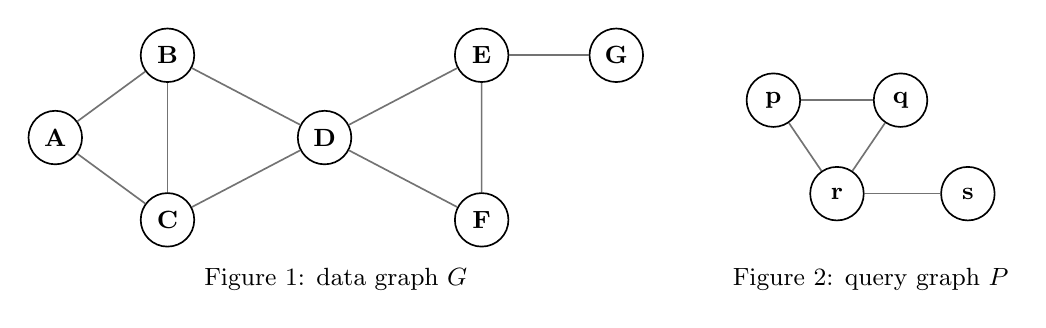
\begin{tikzpicture}[scale=0.95]
  \node[gv] (A) at (0,0)      {A};
  \node[gv] (B) at (1.5,1.1)  {B};
  \node[gv] (C) at (1.5,-1.1) {C};
  \node[gv] (D) at (3.6,0)    {D};
  \node[gv] (E) at (5.7,1.1)  {E};
  \node[gv] (F) at (5.7,-1.1) {F};
  \node[gv] (G) at (7.5,1.1)  {G};
  \foreach \u/\v in {A/B,A/C,B/C,B/D,C/D,D/E,D/F,E/F,E/G} \draw[ue] (\u)--(\v);
  \node[font=\small] at (3.75,-1.9) {Figure 1: data graph $G$};
  \begin{scope}[xshift=9.6cm, yshift=-0.25cm]
    \node[gv] (p) at (0,0.75)    {p};
    \node[gv] (q) at (1.7,0.75)  {q};
    \node[gv] (r) at (0.85,-0.5) {r};
    \node[gv] (s) at (2.6,-0.5)  {s};
    \foreach \u/\v in {p/q,p/r,q/r,r/s} \draw[ue] (\u)--(\v);
    \node[font=\small] at (1.3,-1.65) {Figure 2: query graph $P$};
  \end{scope}
\end{tikzpicture}
\end{center}
\figdata{$E(G)=\{A{-}B,\,A{-}C,\,B{-}C,\,B{-}D,\,C{-}D,\,D{-}E,\,D{-}F,\,E{-}F,\,E{-}G\}$
\quad(9 edges);\qquad $E(P)=\{p{-}q,\,p{-}r,\,q{-}r,\,r{-}s\}$ \quad(4 edges).}

\subsection*{(a) A homomorphism from $P$ to $G$}

A homomorphism only has to map every \emph{edge} of $P$ to an edge of $G$, and distinct
vertices of $P$ may collapse onto one vertex of $G$ --- but only \emph{non-adjacent} ones:
$G$ is simple, so an edge of $P$ whose two endpoints collapsed would need a self-loop in
$G$. Hence $p,q,r$, being pairwise adjacent, must land on three \emph{distinct} vertices
spanning a triangle of $G$, while the pendant $s$ is free to reuse the image of $p$ or $q$.
Sending the triangle to $B,C,D$ leaves $r$'s image $D$ with the spare neighbour $E$ for
$s$, so nothing needs to collapse at all:
\[
  p\mapsto B,\qquad q\mapsto C,\qquad r\mapsto D,\qquad s\mapsto E .
\]

\begin{center}
\rowcolors{2}{accent!6}{white}
\begin{tabular}{l c c c c}
\toprule
\rowcolor{white}
Edge of $P$  & $p$--$q$ & $p$--$r$ & $q$--$r$ & $r$--$s$ \\
\midrule
Image in $G$ & $B$--$C$ \checkmark & $B$--$D$ \checkmark & $C$--$D$ \checkmark & $D$--$E$ \checkmark \\
\bottomrule
\end{tabular}
\end{center}

\answer{A homomorphism from $P$ to $G$ exists, e.g.\ $p\mapsto B$, $q\mapsto C$,
$r\mapsto D$, $s\mapsto E$ (all four edges of $P$ land on edges of $G$).}

\subsection*{(b) All induced subgraphs of $G$ isomorphic to $P$}

$P$ is a triangle plus one pendant vertex ($4$ vertices, $4$ edges). A vertex set
$S\subseteq V(G)$ with $|S|=4$ induces a copy of $P$ \textbf{iff} three of its vertices
form a triangle and the fourth sends \emph{exactly one} edge into that triangle. An induced
subgraph keeps \emph{every} edge of $G$ inside $S$, so two or three such edges would give
$5$ or $6$ edges rather than $4$, whereas zero edges would leave the fourth vertex isolated
even though $P$ is connected. Conversely any induced copy of $P$ must contain a triangle, since $P$ does,
and its remaining vertex is $P$'s degree-$1$ pendant --- so enumerating $G$'s triangles is
exhaustive.

$G$ has exactly three triangles: $\{A,B,C\}$, $\{B,C,D\}$, $\{D,E,F\}$. Extending each by
a fourth vertex:

\begin{center}
\rowcolors{2}{accent!6}{white}
\begin{tabular}{l c l c}
\toprule
\rowcolor{white}
Triangle & 4th vertex & Edges into the triangle & Induced copy of $P$? \\
\midrule
$\{A,B,C\}$ & $D$ & $D$--$B$, $D$--$C$ \quad(2) & no \\
$\{A,B,C\}$ & $E$ & --- \quad(0) & no \\
$\{A,B,C\}$ & $F$ & --- \quad(0) & no \\
$\{A,B,C\}$ & $G$ & --- \quad(0) & no \\
$\{B,C,D\}$ & $A$ & $A$--$B$, $A$--$C$ \quad(2) & no \\
$\{B,C,D\}$ & $E$ & $E$--$D$ \quad(1) & \textbf{yes} \\
$\{B,C,D\}$ & $F$ & $F$--$D$ \quad(1) & \textbf{yes} \\
$\{B,C,D\}$ & $G$ & --- \quad(0) & no \\
$\{D,E,F\}$ & $A$ & --- \quad(0) & no \\
$\{D,E,F\}$ & $B$ & $B$--$D$ \quad(1) & \textbf{yes} \\
$\{D,E,F\}$ & $C$ & $C$--$D$ \quad(1) & \textbf{yes} \\
$\{D,E,F\}$ & $G$ & $G$--$E$ \quad(1) & \textbf{yes} \\
\bottomrule
\end{tabular}
\end{center}

\answer{Exactly five vertex sets induce a subgraph isomorphic to $P$:
$\{B,C,D,E\}$, $\{B,C,D,F\}$, $\{B,D,E,F\}$, $\{C,D,E,F\}$, $\{D,E,F,G\}$.}

%=====================================================================
\needspace{7\baselineskip}
\section*{Q2. Weisfeiler-Lehman color refinement}

\begin{center}
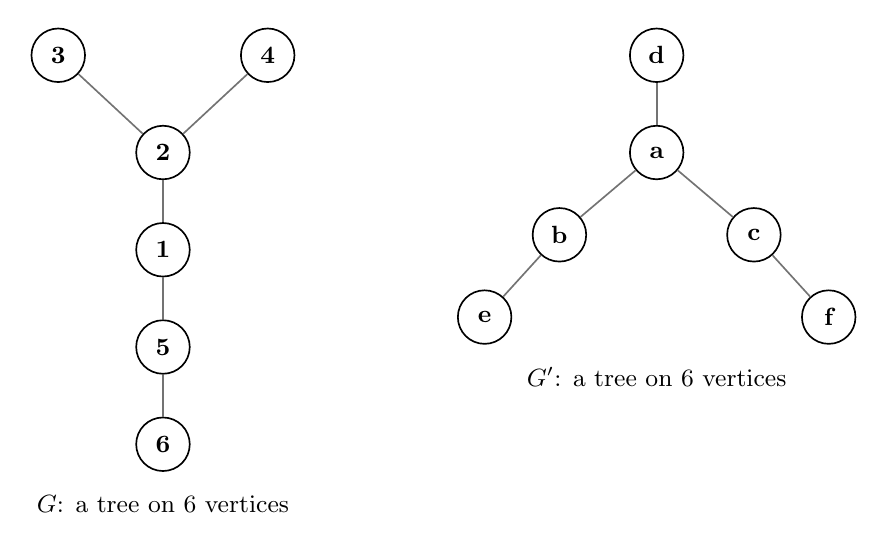
\begin{tikzpicture}[scale=0.95]
  \node[gv] (v2) at (0,0)      {2};
  \node[gv] (v3) at (-1.4,1.3) {3};
  \node[gv] (v4) at (1.4,1.3)  {4};
  \node[gv] (v1) at (0,-1.3)   {1};
  \node[gv] (v5) at (0,-2.6)   {5};
  \node[gv] (v6) at (0,-3.9)   {6};
  \foreach \u/\v in {v2/v3,v2/v4,v2/v1,v1/v5,v5/v6} \draw[ue] (\u)--(\v);
  \node[font=\small] at (0,-4.7) {$G$: a tree on 6 vertices};
  \begin{scope}[xshift=6.6cm]
    \node[gv] (na) at (0,0)       {a};
    \node[gv] (nd) at (0,1.3)     {d};
    \node[gv] (nb) at (-1.3,-1.1) {b};
    \node[gv] (ne) at (-2.3,-2.2) {e};
    \node[gv] (nc) at (1.3,-1.1)  {c};
    \node[gv] (nf) at (2.3,-2.2)  {f};
    \foreach \u/\v in {na/nd,na/nb,na/nc,nb/ne,nc/nf} \draw[ue] (\u)--(\v);
    \node[font=\small] at (0,-3.0) {$G'$: a tree on 6 vertices};
  \end{scope}
\end{tikzpicture}
\end{center}
\figdata{$E(G)=\{1{-}2,\,1{-}5,\,2{-}3,\,2{-}4,\,5{-}6\}$;\qquad
$E(G')=\{a{-}b,\,a{-}c,\,a{-}d,\,b{-}e,\,c{-}f\}$ \quad(5 edges each).}

Both are trees on $6$ vertices with the same degree sequence $[3,2,2,1,1,1]$, so degrees
alone cannot tell them apart.

\noindent\textbf{\color{accent!85!black}Convention.} A vertex's tuple is
$(\text{own colour},\ \text{sorted multiset of neighbour colours})$. Each round, the
distinct tuples occurring in \emph{either} graph are sorted lexicographically and receive
the IDs $0,1,2,\dots$ Restarting the IDs at $0$ in every round is what ``starting from
$0$'' prescribes. Continuing the numbering across rounds instead would only shift each
round's IDs by a constant, padding the vectors with zero entries for the colours of earlier
rounds; since $\boldsymbol{\phi}_t(G)$ and $\boldsymbol{\phi}_t(G')$ are always indexed the
same way, every inner product --- and hence the kernel --- is unchanged either way.

\subsection*{Round 0}

Every vertex has colour $0$, so there is one colour and
$\boldsymbol{\phi}_0(G)=\boldsymbol{\phi}_0(G')=[\,6\,]$.

\subsection*{Round 1}

Lexicographic order of the tuples: $(0,[0])<(0,[0,0])<(0,[0,0,0])$. (Comparing the colour
first and then the neighbour list, or flattening each tuple into one sequence, give the
same order in both rounds, so the answer does not depend on which reading is taken.)

\begin{center}
\rowcolors{2}{accent!6}{white}
\begin{tabular}{c l l}
\toprule
\rowcolor{white}
ID & Tuple & Meaning \\
\midrule
$0$ & $(0,[0])$ & degree-1 vertices \\
$1$ & $(0,[0,0])$ & degree-2 vertices \\
$2$ & $(0,[0,0,0])$ & degree-3 vertices \\
\bottomrule
\end{tabular}
\end{center}

\begin{center}
\rowcolors{2}{accent!6}{white}
\begin{tabular}{c l c}
\toprule
\rowcolor{white}
$G$ & Tuple & New colour \\
\midrule
$1$ & $(0,[0,0])$   & $1$ \\
$2$ & $(0,[0,0,0])$ & $2$ \\
$3$ & $(0,[0])$     & $0$ \\
$4$ & $(0,[0])$     & $0$ \\
$5$ & $(0,[0,0])$   & $1$ \\
$6$ & $(0,[0])$     & $0$ \\
\bottomrule
\end{tabular}
\qquad
\rowcolors{2}{accent!6}{white}
\begin{tabular}{c l c}
\toprule
\rowcolor{white}
$G'$ & Tuple & New colour \\
\midrule
$a$ & $(0,[0,0,0])$ & $2$ \\
$b$ & $(0,[0,0])$   & $1$ \\
$c$ & $(0,[0,0])$   & $1$ \\
$d$ & $(0,[0])$     & $0$ \\
$e$ & $(0,[0])$     & $0$ \\
$f$ & $(0,[0])$     & $0$ \\
\bottomrule
\end{tabular}
\end{center}

\[
  \boldsymbol{\phi}_1(G)=[\,3,2,1\,],\qquad \boldsymbol{\phi}_1(G')=[\,3,2,1\,]
\]
still identical --- round $1$ only counts degrees.

\subsection*{Round 2}

Tuples are built from the round-1 colours above.

\begin{center}
\rowcolors{2}{accent!6}{white}
\begin{tabular}{c c l l c}
\toprule
\rowcolor{white}
$G$ & Colour & Neighbours' colours & Tuple & New colour \\
\midrule
$1$ & $1$ & $2(2),\,5(1)$          & $(1,[1,2])$   & $4$ \\
$2$ & $2$ & $1(1),\,3(0),\,4(0)$   & $(2,[0,0,1])$ & $5$ \\
$3$ & $0$ & $2(2)$                 & $(0,[2])$     & $1$ \\
$4$ & $0$ & $2(2)$                 & $(0,[2])$     & $1$ \\
$5$ & $1$ & $1(1),\,6(0)$          & $(1,[0,1])$   & $2$ \\
$6$ & $0$ & $5(1)$                 & $(0,[1])$     & $0$ \\
\bottomrule
\end{tabular}
\end{center}

\begin{center}
\rowcolors{2}{accent!6}{white}
\begin{tabular}{c c l l c}
\toprule
\rowcolor{white}
$G'$ & Colour & Neighbours' colours & Tuple & New colour \\
\midrule
$a$ & $2$ & $b(1),\,c(1),\,d(0)$ & $(2,[0,1,1])$ & $6$ \\
$b$ & $1$ & $a(2),\,e(0)$        & $(1,[0,2])$   & $3$ \\
$c$ & $1$ & $a(2),\,f(0)$        & $(1,[0,2])$   & $3$ \\
$d$ & $0$ & $a(2)$               & $(0,[2])$     & $1$ \\
$e$ & $0$ & $b(1)$               & $(0,[1])$     & $0$ \\
$f$ & $0$ & $c(1)$               & $(0,[1])$     & $0$ \\
\bottomrule
\end{tabular}
\end{center}

Seven distinct tuples occur across the two graphs; sorted lexicographically they receive
the IDs $0$--$6$:

\noindent\begin{minipage}{\linewidth}
\begin{center}
\rowcolors{2}{accent!6}{white}
\begin{tabular}{c l c c}
\toprule
\rowcolor{white}
ID & Tuple & Count in $G$ & Count in $G'$ \\
\midrule
$0$ & $(0,[1])$     & $1$ & $2$ \\
$1$ & $(0,[2])$     & $2$ & $1$ \\
$2$ & $(1,[0,1])$   & $1$ & $0$ \\
$3$ & $(1,[0,2])$   & $0$ & $2$ \\
$4$ & $(1,[1,2])$   & $1$ & $0$ \\
$5$ & $(2,[0,0,1])$ & $1$ & $0$ \\
$6$ & $(2,[0,1,1])$ & $0$ & $1$ \\
\midrule
\rowcolor{white}
\multicolumn{2}{r}{\textbf{total}} & $6$ & $6$ \\
\bottomrule
\end{tabular}
\end{center}
\end{minipage}

\[
  \boldsymbol{\phi}_2(G)=[\,1,2,1,0,1,1,0\,],\qquad
  \boldsymbol{\phi}_2(G')=[\,2,1,0,2,0,0,1\,]
\]

Round $2$ is the first round that separates the two trees: in $G$ the degree-3 vertex sees
two leaves and one degree-2 vertex, whereas in $G'$ it sees one leaf and two degree-2
vertices.

\subsection*{(b) The two-round WL kernel}

\begin{center}
\rowcolors{2}{accent!6}{white}
\begin{tabular}{c l l l}
\toprule
\rowcolor{white}
$t$ & $\boldsymbol{\phi}_t(G)$ & $\boldsymbol{\phi}_t(G')$ & $\boldsymbol{\phi}_t(G)^{\mathsf T}\boldsymbol{\phi}_t(G')$ \\
\midrule
$0$ & $[6]$ & $[6]$ & $6\cdot 6=36$ \\
$1$ & $[3,2,1]$ & $[3,2,1]$ & $9+4+1=14$ \\
$2$ & $[1,2,1,0,1,1,0]$ & $[2,1,0,2,0,0,1]$ & $1\cdot 2+2\cdot 1=4$ \\
\bottomrule
\end{tabular}
\end{center}

\answer{$K_{\mathrm{WL}}(G,G')=36+14+4=\mathbf{54}$.}

%=====================================================================
\needspace{7\baselineskip}
\section*{Q3. Reachability indexing}

\subsection*{(a) Minimal 2-hop labelling}

\begin{center}
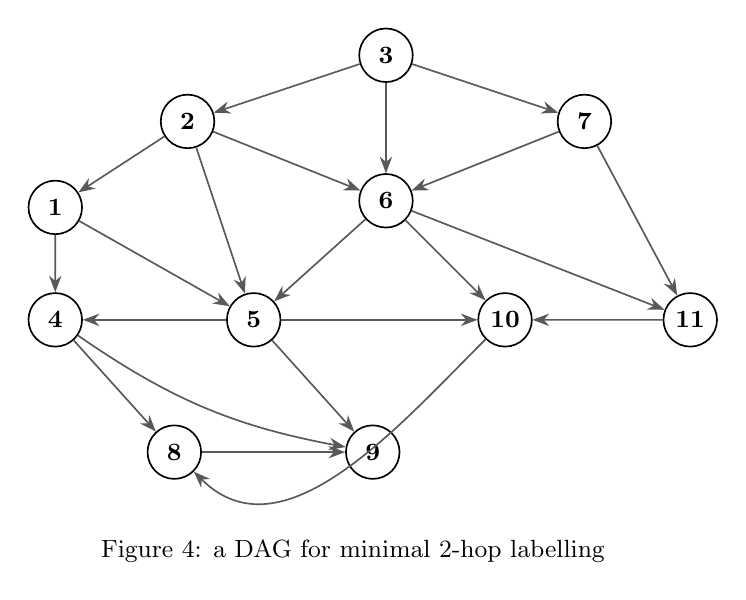
\begin{tikzpicture}[scale=0.84]
  \node[gv] (n3)  at (7,7)    {3};
  \node[gv] (n2)  at (4,6)    {2};
  \node[gv] (n7)  at (10,6)   {7};
  \node[gv] (n1)  at (2,4.7)  {1};
  \node[gv] (n6)  at (7,4.8)  {6};
  \node[gv] (n4)  at (2,3)    {4};
  \node[gv] (n5)  at (5,3)    {5};
  \node[gv] (n10) at (8.8,3)  {10};
  \node[gv] (n11) at (11.6,3) {11};
  \node[gv] (n8)  at (3.8,1)  {8};
  \node[gv] (n9)  at (6.8,1)  {9};
  \foreach \u/\v in {n1/n4,n1/n5,n2/n1,n2/n5,n2/n6,n3/n2,n3/n6,n3/n7,
                     n4/n8,n5/n4,n5/n9,n5/n10,n6/n5,n6/n10,n6/n11,
                     n7/n6,n7/n11,n8/n9,n11/n10}
    \draw[de] (\u)--(\v);
  \draw[de] (n4) to[bend right=12] (n9);
  \draw[de] (n10) to[out=225,in=315] (n8);
  \node[font=\small] at (6.5,-0.5) {Figure 4: a DAG for minimal 2-hop labelling};
\end{tikzpicture}
\end{center}
\figdata{Edges (21):
$1{\to}4$, $1{\to}5$, $2{\to}1$, $2{\to}5$, $2{\to}6$, $3{\to}2$, $3{\to}6$,
$3{\to}7$, $4{\to}8$, $4{\to}9$, $5{\to}4$, $5{\to}9$, $5{\to}10$, $6{\to}5$,
$6{\to}10$, $6{\to}11$, $7{\to}6$, $7{\to}11$, $8{\to}9$, $10{\to}8$, $11{\to}10$.}

\noindent\textbf{\color{accent!85!black}Convention.} $L_{\mathrm{out}}(u)$ holds hubs
reachable \emph{from} $u$, $L_{\mathrm{in}}(v)$ holds hubs that \emph{reach} $v$, and
\[
  u\rightsquigarrow v \iff L_{\mathrm{out}}(u)\cap L_{\mathrm{in}}(v)\neq\emptyset .
\]
Every vertex ends up in its own two labels. This is not a convention chosen by hand --- it
follows from the algorithm below. Each of hub $k$'s two searches starts \emph{at $k$}, and
the pruning test there is whether $L_{\mathrm{out}}(k)\cap L_{\mathrm{in}}(k)$ is already
non-empty. In a DAG that intersection is necessarily empty before $k$ labels itself: a
common hub $h\neq k$ would give $k\rightsquigarrow h$ and $h\rightsquigarrow k$, i.e.\ a
cycle. So $k$ is never pruned at itself and always adds
$k\in L_{\mathrm{out}}(k)$, $k\in L_{\mathrm{in}}(k)$. This is also exactly what makes the
reflexive query $v\rightsquigarrow v$ answerable, since $v$ is the only possible hub for it.

\noindent\textbf{\color{accent!85!black}Processing order.} Total degree $=$ in-degree $+$
out-degree, decreasing, ties broken by smaller vertex ID:

\begin{center}
\rowcolors{2}{accent!6}{white}
\begin{tabular}{l c c c c c c c c c c c}
\toprule
\rowcolor{white}
$v$ & $1$ & $2$ & $3$ & $4$ & $5$ & $6$ & $7$ & $8$ & $9$ & $10$ & $11$ \\
\midrule
in-degree  & $1$ & $1$ & $0$ & $2$ & $3$ & $3$ & $1$ & $2$ & $3$ & $3$ & $2$ \\
out-degree & $2$ & $3$ & $3$ & $2$ & $3$ & $3$ & $2$ & $1$ & $0$ & $1$ & $1$ \\
\textbf{total} & $3$ & $4$ & $3$ & $4$ & $\mathbf{6}$ & $\mathbf{6}$ & $3$ & $3$ & $3$ & $4$ & $3$ \\
\bottomrule
\end{tabular}
\end{center}

\[
  \text{Order:}\quad 5,\;6,\;2,\;4,\;10,\;1,\;3,\;7,\;8,\;9,\;11
\]

\noindent\textbf{\color{accent!85!black}Algorithm.} Take the hubs $k$ in that order. For
each $k$ run a \emph{backward} BFS (over reversed edges) and a \emph{forward} BFS. On
reaching a vertex $x$, first test whether the labels built \emph{so far} already prove the
corresponding reachability --- $L_{\mathrm{out}}(x)\cap L_{\mathrm{in}}(k)\neq\emptyset$
backward, $L_{\mathrm{out}}(k)\cap L_{\mathrm{in}}(x)\neq\emptyset$ forward. If they do,
\textbf{prune}: add nothing and do not expand past $x$. This is sound because the hub $h$
that certifies the pair was processed \emph{earlier} and lies on the path from $k$ through
$x$ to everything beyond it, so each of those pairs is already answered by the labels built
so far --- though not necessarily through $h$ itself. (At hub $2$, for instance, the
forward BFS prunes at $6$ via hub $6$, yet the pair $2\rightsquigarrow 4$ behind it is
certified by hub $5$.) Otherwise add $k$ to $L_{\mathrm{out}}(x)$
(backward) or $L_{\mathrm{in}}(x)$ (forward) and keep expanding. The result is a
\emph{minimal} $2$-hop cover: no single entry can be deleted without breaking some
reachable pair.

\medskip
\noindent\textbf{Round-by-round trace} ($+v$ = hub added at $v$, $\times v$ = pruned at $v$):

\begin{center}
\rowcolors{2}{accent!6}{white}
\begin{tabular}{c l l}
\toprule
\rowcolor{white}
Hub $k$ & Backward BFS $\rightarrow L_{\mathrm{out}}$ & Forward BFS $\rightarrow L_{\mathrm{in}}$ \\
\midrule
$5$  & $+1,+2,+3,+5,+6,+7$ & $+4,+5,+8,+9,+10$ \\
$6$  & $+2,+3,+6,+7$ & $+6,+11$;\quad $\times 5,\times 10$ \\
$2$  & $+2,+3$ & $+1,+2$;\quad $\times 4,\times 5,\times 6$ \\
$4$  & $+4$;\quad $\times 1,\times 5$ & $+4,+8,+9$ \\
$10$ & $+10,+11$;\quad $\times 5,\times 6,\times 7$ & $+8,+9,+10$ \\
$1$  & $+1$;\quad $\times 2$ & $+1$;\quad $\times 4,\times 5$ \\
$3$  & $+3$ & $+3,+7$;\quad $\times 2,\times 6,\times 11$ \\
$7$  & $+7$;\quad $\times 3$ & $+7$;\quad $\times 6,\times 11$ \\
$8$  & $+8$;\quad $\times 4,\times 10$ & $+8,+9$ \\
$9$  & $+9$;\quad $\times 4,\times 5,\times 8$ & $+9$ \\
$11$ & $+11$;\quad $\times 6,\times 7$ & $+11$;\quad $\times 10$ \\
\bottomrule
\end{tabular}
\end{center}

\noindent Two examples of the pruning. At hub $6$ the forward BFS stops at $5$ because
$5\in L_{\mathrm{out}}(6)$ and $5\in L_{\mathrm{in}}(5)$ already certify $6\rightsquigarrow 5$;
everything behind $5$ (namely $4,8,9,10$) happens to be covered through hub $5$ as well ---
this is one of the cases where the certifying hub does cover the whole tail --- so the
search need not go on. At hub $8$ the backward BFS stops at $4$ and at $10$, whose labels
$L_{\mathrm{out}}(4)=\{4\}$ and $L_{\mathrm{out}}(10)=\{10\}$ already meet
$L_{\mathrm{in}}(8)=\{4,5,10\}$.

\medskip
\noindent\begin{minipage}{\linewidth}
\noindent\textbf{Final labels.}

\begin{center}
\rowcolors{2}{accent!6}{white}
\begin{tabular}{c l l}
\toprule
\rowcolor{white}
$v$ & $L_{\mathrm{in}}(v)$ & $L_{\mathrm{out}}(v)$ \\
\midrule
$1$  & $\{1,2\}$          & $\{1,5\}$ \\
$2$  & $\{2\}$            & $\{2,5,6\}$ \\
$3$  & $\{3\}$            & $\{2,3,5,6\}$ \\
$4$  & $\{4,5\}$          & $\{4\}$ \\
$5$  & $\{5\}$            & $\{5\}$ \\
$6$  & $\{6\}$            & $\{5,6\}$ \\
$7$  & $\{3,7\}$          & $\{5,6,7\}$ \\
$8$  & $\{4,5,8,10\}$     & $\{8\}$ \\
$9$  & $\{4,5,8,9,10\}$   & $\{9\}$ \\
$10$ & $\{5,10\}$         & $\{10\}$ \\
$11$ & $\{6,11\}$         & $\{10,11\}$ \\
\midrule
\rowcolor{white}
\textbf{total} & $23$ entries & $21$ entries \\
\bottomrule
\end{tabular}
\end{center}
\end{minipage}

\noindent Sanity checks: $3\rightsquigarrow 9$ because
$L_{\mathrm{out}}(3)\cap L_{\mathrm{in}}(9)=\{5\}$ (indeed $3\to 2\to 5\to 9$);
$1\not\rightsquigarrow 11$ because $L_{\mathrm{out}}(1)\cap L_{\mathrm{in}}(11)
=\{1,5\}\cap\{6,11\}=\emptyset$, and everything reachable from $1$ does stay inside
$\{4,5,8,9,10\}$.

\answer{The minimal 2-hop labels are the $44$ entries tabulated above (23 in $L_{\mathrm{in}}$,
21 in $L_{\mathrm{out}}$), obtained by pruned BFS with the hub order
$5,6,2,4,10,1,3,7,8,9,11$.}

\subsection*{(b) Comparing two spanning trees}

\begin{center}
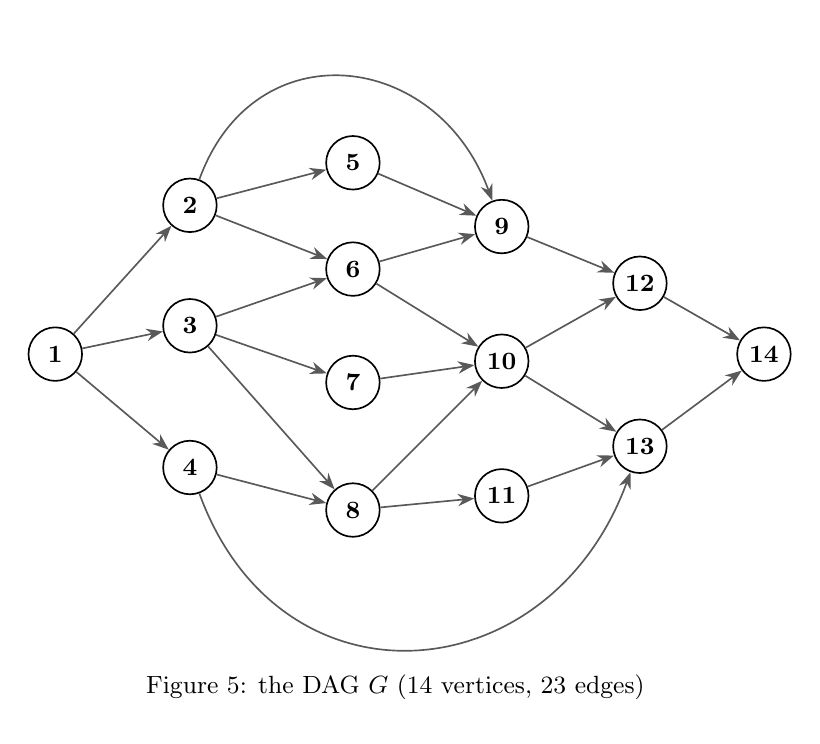
\begin{tikzpicture}[scale=0.9]
  \node[gv] (m1)  at (0.7,2.2)  {1};
  \node[gv] (m2)  at (2.6,4.3)  {2};
  \node[gv] (m3)  at (2.6,2.6)  {3};
  \node[gv] (m4)  at (2.6,0.6)  {4};
  \node[gv] (m5)  at (4.9,4.9)  {5};
  \node[gv] (m6)  at (4.9,3.4)  {6};
  \node[gv] (m7)  at (4.9,1.8)  {7};
  \node[gv] (m8)  at (4.9,0)    {8};
  \node[gv] (m9)  at (7.0,4.0)  {9};
  \node[gv] (m10) at (7.0,2.1)  {10};
  \node[gv] (m11) at (7.0,0.2)  {11};
  \node[gv] (m12) at (8.95,3.2) {12};
  \node[gv] (m13) at (8.95,0.9) {13};
  \node[gv] (m14) at (10.7,2.2) {14};
  \foreach \u/\v in {m1/m2,m1/m3,m1/m4,m2/m5,m2/m6,m3/m6,m3/m7,m3/m8,
                     m4/m8,m5/m9,m6/m9,m6/m10,m7/m10,m8/m10,m8/m11,
                     m9/m12,m10/m12,m10/m13,m11/m13,m12/m14,m13/m14}
    \draw[de] (\u)--(\v);
  \draw[de] (m2) to[out=70,in=110,looseness=1.4] (m9);
  \draw[de] (m4) to[out=-70,in=-110,looseness=1.4] (m13);
  \node[font=\small] at (5.5,-2.5) {Figure 5: the DAG $G$ (14 vertices, 23 edges)};
\end{tikzpicture}
\end{center}
\figdata{Edges (23; vertex 1 is the only source):
$1{\to}2$, $1{\to}3$, $1{\to}4$, $2{\to}5$, $2{\to}6$, $2{\to}9$, $3{\to}6$,
$3{\to}7$, $3{\to}8$, $4{\to}8$, $4{\to}13$, $5{\to}9$, $6{\to}9$, $6{\to}10$,
$7{\to}10$, $8{\to}10$, $8{\to}11$, $9{\to}12$, $10{\to}12$, $10{\to}13$,
$11{\to}13$, $12{\to}14$, $13{\to}14$.}

\noindent\textbf{\color{accent!85!black}Algorithm.} Number the tree vertices by a
\textbf{left-to-right post-order} traversal. Each vertex $v$ receives the interval
\[
  I(v)=\bigl[\,\min\{\text{post-numbers in }v\text{'s subtree}\},\ \mathrm{post}(v)\,\bigr],
\]
which covers exactly $v$'s tree descendants. Then, in \textbf{reverse topological order},
\[
  L(u)=I(u)\ \cup \bigcup_{u\to w\,\in\,E} L(w),
\]
deleting from $L(u)$ any interval \emph{contained} in another interval of the same label ---
that is the redundancy the algorithm removes. A query is then
$u\rightsquigarrow v \iff \mathrm{post}(v)$ lies in some interval of $L(u)$.

Adjacent or partially overlapping intervals are \emph{not} merged. Merging them would in
fact stay correct, since post-numbers are consecutive integers and e.g.\ $[1,2]$ together
with $[3,6]$ covers exactly $[1,6]$; it is simply a further compression that the tree-cover
algorithm does not perform. It would not affect the comparison either --- merged, the two
labellings below need $25$ and $27$ intervals instead of $26$ and $31$, so Tree~1 still
wins.

Both spanning trees are rooted at vertex $1$, the only source of the DAG. The post-order
number of each vertex is printed in \textcolor{accent}{blue} beside it.

\begin{center}
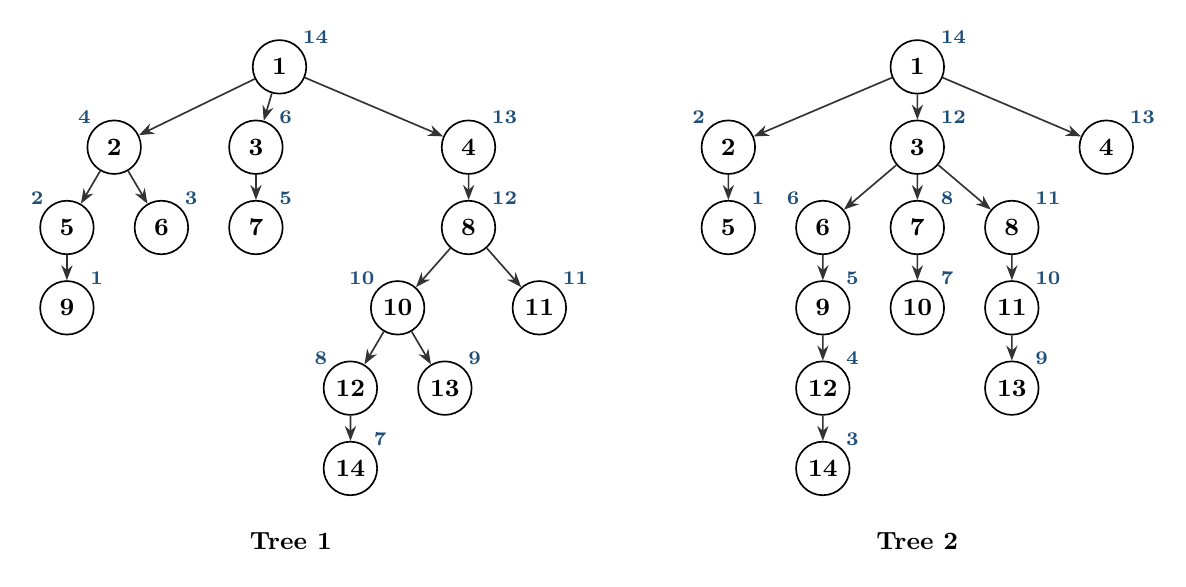
\begin{tikzpicture}[xscale=1.2, yscale=1.02]
  % Post-order numbers sit up-right of each vertex, except where the incoming
  % tree edge arrives from that side -- those are placed up-left instead.
  % ---------------- Tree 1 ----------------
  \node[gv, label={[post]45:14}]  (a1)  at (2.78,0)     {1};
  \node[gv, label={[post]135:4}]  (a2)  at (1.03,-1)    {2};
  \node[gv, label={[post]45:6}]   (a3)  at (2.53,-1)    {3};
  \node[gv, label={[post]45:13}]  (a4)  at (4.78,-1)    {4};
  \node[gv, label={[post]135:2}]  (a5)  at (0.53,-2)    {5};
  \node[gv, label={[post]45:3}]   (a6)  at (1.53,-2)    {6};
  \node[gv, label={[post]45:5}]   (a7)  at (2.53,-2)    {7};
  \node[gv, label={[post]45:12}]  (a8)  at (4.78,-2)    {8};
  \node[gv, label={[post]45:1}]   (a9)  at (0.53,-3)    {9};
  \node[gv, label={[post]135:10}] (a10) at (4.03,-3)    {10};
  \node[gv, label={[post]45:11}]  (a11) at (5.53,-3)    {11};
  \node[gv, label={[post]135:8}]  (a12) at (3.53,-4)    {12};
  \node[gv, label={[post]45:9}]   (a13) at (4.53,-4)    {13};
  \node[gv, label={[post]45:7}]   (a14) at (3.53,-5)    {14};
  \foreach \u/\v in {a1/a2,a1/a3,a1/a4,a2/a5,a2/a6,a3/a7,a4/a8,a5/a9,
                     a8/a10,a8/a11,a10/a12,a10/a13,a12/a14}
    \draw[te] (\u)--(\v);
  \node[font=\small\bfseries] at (2.9,-5.9) {Tree 1};
  % ---------------- Tree 2 ----------------
  \begin{scope}[xshift=7.0cm]
    \node[gv, label={[post]45:14}] (b1)  at (2.53,0)  {1};
    \node[gv, label={[post]135:2}] (b2)  at (0.53,-1) {2};
    \node[gv, label={[post]45:12}] (b3)  at (2.53,-1) {3};
    \node[gv, label={[post]45:13}] (b4)  at (4.53,-1) {4};
    \node[gv, label={[post]45:1}]  (b5)  at (0.53,-2) {5};
    \node[gv, label={[post]135:6}] (b6)  at (1.53,-2) {6};
    \node[gv, label={[post]45:8}]  (b7)  at (2.53,-2) {7};
    \node[gv, label={[post]45:11}] (b8)  at (3.53,-2) {8};
    \node[gv, label={[post]45:5}]  (b9)  at (1.53,-3) {9};
    \node[gv, label={[post]45:7}]  (b10) at (2.53,-3) {10};
    \node[gv, label={[post]45:10}] (b11) at (3.53,-3) {11};
    \node[gv, label={[post]45:4}]  (b12) at (1.53,-4) {12};
    \node[gv, label={[post]45:9}]  (b13) at (3.53,-4) {13};
    \node[gv, label={[post]45:3}]  (b14) at (1.53,-5) {14};
    \foreach \u/\v in {b1/b2,b1/b3,b1/b4,b2/b5,b3/b6,b3/b7,b3/b8,b6/b9,
                       b7/b10,b8/b11,b9/b12,b11/b13,b12/b14}
      \draw[te] (\u)--(\v);
    \node[font=\small\bfseries] at (2.53,-5.9) {Tree 2};
  \end{scope}
\end{tikzpicture}
\end{center}
\figdata{Children, left to right ---\\
Tree 1: $1{:}\,2,3,4$; $2{:}\,5,6$; $3{:}\,7$; $4{:}\,8$; $5{:}\,9$; $8{:}\,10,11$;
$10{:}\,12,13$; $12{:}\,14$.\\
Tree 2: $1{:}\,2,3,4$; $2{:}\,5$; $3{:}\,6,7,8$; $6{:}\,9$; $7{:}\,10$; $8{:}\,11$;
$9{:}\,12$; $11{:}\,13$; $12{:}\,14$.}

\noindent\begin{minipage}{\linewidth}
\noindent\textbf{Tree 1.} Post-order: $9,5,6,2,7,3,14,12,13,10,11,8,4,1$.

\begin{center}
\rowcolors{2}{accent!6}{white}
\begin{tabular}{c c c l c}
\toprule
\rowcolor{white}
$v$ & post & $I(v)$ & Final $L(v)$ & $|L(v)|$ \\
\midrule
$1$  & $14$ & $[1,14]$   & $[1,14]$ & $1$ \\
$2$  & $4$  & $[1,4]$    & $[1,4],\,[7,10]$ & $2$ \\
$3$  & $6$  & $[5,6]$    & $[1,1],\,[3,3],\,[5,6],\,[7,12]$ & $4$ \\
$4$  & $13$ & $[7,13]$   & $[7,13]$ & $1$ \\
$5$  & $2$  & $[1,2]$    & $[1,2],\,[7,8]$ & $2$ \\
$6$  & $3$  & $[3,3]$    & $[1,1],\,[3,3],\,[7,10]$ & $3$ \\
$7$  & $5$  & $[5,5]$    & $[5,5],\,[7,10]$ & $2$ \\
$8$  & $12$ & $[7,12]$   & $[7,12]$ & $1$ \\
$9$  & $1$  & $[1,1]$    & $[1,1],\,[7,8]$ & $2$ \\
$10$ & $10$ & $[7,10]$   & $[7,10]$ & $1$ \\
$11$ & $11$ & $[11,11]$  & $[7,7],\,[9,9],\,[11,11]$ & $3$ \\
$12$ & $8$  & $[7,8]$    & $[7,8]$ & $1$ \\
$13$ & $9$  & $[9,9]$    & $[7,7],\,[9,9]$ & $2$ \\
$14$ & $7$  & $[7,7]$    & $[7,7]$ & $1$ \\
\midrule
\rowcolor{white}
\multicolumn{4}{r}{\textbf{Total intervals}} & $\mathbf{26}$ \\
\bottomrule
\end{tabular}
\end{center}
\end{minipage}

\noindent\begin{minipage}{\linewidth}
\noindent\textbf{Tree 2.} Post-order: $5,2,14,12,9,6,10,7,13,11,8,3,4,1$.

\begin{center}
\rowcolors{2}{accent!6}{white}
\begin{tabular}{c c c l c}
\toprule
\rowcolor{white}
$v$ & post & $I(v)$ & Final $L(v)$ & $|L(v)|$ \\
\midrule
$1$  & $14$ & $[1,14]$  & $[1,14]$ & $1$ \\
$2$  & $2$  & $[1,2]$   & $[1,2],\,[3,6],\,[7,7],\,[9,9]$ & $4$ \\
$3$  & $12$ & $[3,12]$  & $[3,12]$ & $1$ \\
$4$  & $13$ & $[13,13]$ & $[3,4],\,[7,7],\,[9,11],\,[13,13]$ & $4$ \\
$5$  & $1$  & $[1,1]$   & $[1,1],\,[3,5]$ & $2$ \\
$6$  & $6$  & $[3,6]$   & $[3,6],\,[7,7],\,[9,9]$ & $3$ \\
$7$  & $8$  & $[7,8]$   & $[3,4],\,[7,8],\,[9,9]$ & $3$ \\
$8$  & $11$ & $[9,11]$  & $[3,4],\,[7,7],\,[9,11]$ & $3$ \\
$9$  & $5$  & $[3,5]$   & $[3,5]$ & $1$ \\
$10$ & $7$  & $[7,7]$   & $[3,4],\,[7,7],\,[9,9]$ & $3$ \\
$11$ & $10$ & $[9,10]$  & $[3,3],\,[9,10]$ & $2$ \\
$12$ & $4$  & $[3,4]$   & $[3,4]$ & $1$ \\
$13$ & $9$  & $[9,9]$   & $[3,3],\,[9,9]$ & $2$ \\
$14$ & $3$  & $[3,3]$   & $[3,3]$ & $1$ \\
\midrule
\rowcolor{white}
\multicolumn{4}{r}{\textbf{Total intervals}} & $\mathbf{31}$ \\
\bottomrule
\end{tabular}
\end{center}
\end{minipage}

\noindent\begin{minipage}{\linewidth}
\subsubsection*{Which tree gives the better labelling?}

\begin{center}
\rowcolors{2}{accent!6}{white}
\begin{tabular}{l c c}
\toprule
\rowcolor{white}
 & \textbf{Tree 1} & \textbf{Tree 2} \\
\midrule
Total intervals (index size) & $\mathbf{26}$ & $31$ \\
Largest single label & $4$ (vertex $3$) & $4$ (vertices $2,4$) \\
Vertices with a single interval & $6$ \ ($1,4,8,10,12,14$) & $5$ \ ($1,3,9,12,14$) \\
Label-size distribution ($1/2/3/4$) & $6/5/2/1$ & $5/3/4/2$ \\
Non-tree edges absorbed at no cost & $2$ \ ($2\to 9$, $4\to 13$) & $0$ \\
\bottomrule
\end{tabular}
\end{center}
\end{minipage}

\noindent\textbf{\color{accent!85!black}Why.} A vertex's label starts as its own interval
and then grows by inheriting intervals along its out-edges. Two distinct effects limit that
growth.

\begin{itemize}[nosep,leftmargin=1.3em]
  \item A non-tree edge $u\to w$ is \emph{free} whenever $w$ is already a tree descendant
    of $u$, because the tree path from $u$ down to $w$ carries $L(w)$ upward in any case.
    Note this is \emph{not} a containment effect: in Tree 1, $L(9)=\{[1,1],[7,8]\}$ is not
    inside $I(2)=[1,4]$, yet the edge $2\to 9$ still costs nothing.
  \item Containment is the stronger effect, and the one that decides this comparison. If
    everything $u$ can reach lies inside $u$'s own subtree, then every inherited interval
    has both endpoints among that subtree's post-numbers, so it is contained in $I(u)$ and
    deleted --- and $L(u)$ collapses to the single interval $I(u)$. In both trees
    $L(u)=\{I(u)\}$ holds \emph{exactly} for the vertices counted in the
    ``single interval'' row above.
\end{itemize}

\noindent So a spanning tree is good precisely when it keeps mutually reachable clusters
together inside one subtree. Applying that to the two spanning trees:

\begin{itemize}[nosep,leftmargin=1.3em]
  \item \textbf{Tree 1} puts the DAG's whole converging tail --- $4,8,10,11,12,13,14$ ---
    into a single subtree rooted at $4$ ($4\to 8\to\{10,11\}$, $10\to\{12,13\}$,
    $12\to 14$). Every DAG edge among those vertices therefore stays inside that subtree,
    so $L(4)$ collapses to the one interval $[7,13]$, and likewise $L(8)=[7,12]$,
    $L(10)=[7,10]$, $L(12)=[7,8]$. On top of that, the non-tree edges $2\to 9$ and
    $4\to 13$ point back into the subtree they start from and cost nothing at all.
  \item \textbf{Tree 2} splits that same tail across three sibling branches of vertex $3$
    ($6\to 9\to 12\to 14$, $7\to 10$, $8\to 11\to 13$) and leaves vertex $4$ as a
    \emph{leaf}. A leaf's interval $I(4)=[13,13]$ is a single point that can absorb
    nothing, so $4\to 8$ and $4\to 13$ push $L(4)$ up to four intervals. The cross-branch
    edges $6\to 10$, $8\to 10$, $10\to 12$, $10\to 13$ and $13\to 14$ are likewise all
    non-tree edges between \emph{different} branches, so their intervals propagate upward
    instead of being swallowed. That is why six of Tree 2's vertices need three or four
    intervals, against three in Tree 1.
\end{itemize}

\noindent Note that the \emph{maximum} label size is $4$ for both trees, so what separates
them is the total index size --- which is also what determines the space used and the cost
of a query, since answering $u\rightsquigarrow v$ scans $L(u)$.

\answer{\textbf{Tree 1} gives the better tree-cover labelling: $26$ intervals against
Tree 2's $31$ ($16\%$ smaller), because Tree 1 keeps the DAG's converging tail
$\{4,8,10,11,12,13,14\}$ inside one subtree, whereas Tree 2 scatters it over three sibling
branches and leaves vertex $4$ as an absorbing-nothing leaf.}

%=====================================================================
\needspace{7\baselineskip}
\section*{Q4. One-layer GNN mean aggregation}

\begin{center}
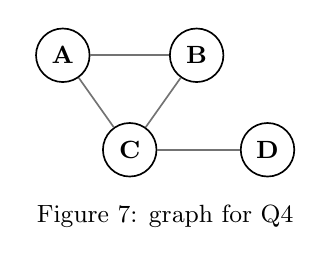
\begin{tikzpicture}[scale=1.0]
  \node[gv] (qA) at (0,1.2)    {A};
  \node[gv] (qB) at (1.7,1.2)  {B};
  \node[gv] (qC) at (0.85,0)   {C};
  \node[gv] (qD) at (2.6,0)    {D};
  \foreach \u/\v in {qA/qB,qA/qC,qB/qC,qC/qD} \draw[ue] (\u)--(\v);
  \node[font=\small] at (1.3,-0.85) {Figure 7: graph for Q4};
\end{tikzpicture}
\end{center}
\figdata{$E=\{A{-}B,\,A{-}C,\,B{-}C,\,C{-}D\}$;\quad
$N(A)=\{B,C\}$, $N(B)=\{A,C\}$, $N(C)=\{A,B,D\}$, $N(D)=\{C\}$.}

\[
  h_A^{(0)}=\begin{pmatrix}1\\0\end{pmatrix},\quad
  h_B^{(0)}=\begin{pmatrix}0\\1\end{pmatrix},\quad
  h_C^{(0)}=\begin{pmatrix}1\\1\end{pmatrix},\quad
  h_D^{(0)}=\begin{pmatrix}2\\0\end{pmatrix},\qquad
  W=\begin{pmatrix}1&-1&1&0\\0&1&-1&1\end{pmatrix}
\]

\subsection*{(a) Vertices $B$ and $C$}

\noindent\textbf{Vertex $B$}, with $N(B)=\{A,C\}$:
\begin{align*}
  h_{N(B)}^{(0)} &= \tfrac12\left[\begin{pmatrix}1\\0\end{pmatrix}
                  + \begin{pmatrix}1\\1\end{pmatrix}\right]
                  = \begin{pmatrix}1\\[2pt] 0.5\end{pmatrix},\qquad
  \mathrm{CONCAT}\bigl(h_B^{(0)},h_{N(B)}^{(0)}\bigr)
                  = (0,\,1,\,1,\,0.5)^{\mathsf T}\\[4pt]
  W\cdot(0,\,1,\,1,\,0.5)^{\mathsf T}
    &= \begin{pmatrix} 1(0)-1(1)+1(1)+0(0.5)\\[2pt] 0(0)+1(1)-1(1)+1(0.5)\end{pmatrix}
     = \begin{pmatrix}0\\[2pt]0.5\end{pmatrix}
  \;\xrightarrow{\ \mathrm{ReLU}\ }\;
  h_B^{(1)}=\begin{pmatrix}0.00\\[2pt]0.50\end{pmatrix}
\end{align*}

\noindent\textbf{Vertex $C$}, with $N(C)=\{A,B,D\}$:
\begin{align*}
  h_{N(C)}^{(0)} &= \tfrac13\left[\begin{pmatrix}1\\0\end{pmatrix}
                  + \begin{pmatrix}0\\1\end{pmatrix}
                  + \begin{pmatrix}2\\0\end{pmatrix}\right]
                  = \begin{pmatrix}1\\[2pt] 1/3\end{pmatrix},\qquad
  \mathrm{CONCAT}\bigl(h_C^{(0)},h_{N(C)}^{(0)}\bigr)
                  = \bigl(1,\,1,\,1,\,\tfrac13\bigr)^{\mathsf T}\\[4pt]
  W\cdot\bigl(1,\,1,\,1,\,\tfrac13\bigr)^{\mathsf T}
    &= \begin{pmatrix} 1-1+1+0\\[2pt] 0+1-1+\tfrac13\end{pmatrix}
     = \begin{pmatrix}1\\[2pt]1/3\end{pmatrix}
  \;\xrightarrow{\ \mathrm{ReLU}\ }\;
  h_C^{(1)}=\begin{pmatrix}1.00\\[2pt]0.33\end{pmatrix}
\end{align*}

\begin{center}
\rowcolors{2}{accent!6}{white}
\begin{tabular}{c c c c c}
\toprule
\rowcolor{white}
$v$ & $N(v)$ & Neighbour mean & Concatenated input & $h_v^{(1)}$ \\
\midrule
$B$ & $\{A,C\}$   & $(1,\ 0.5)^{\mathsf T}$ & $(0,\,1,\,1,\,0.5)^{\mathsf T}$ & $\mathbf{(0.00,\ 0.50)^{\mathsf T}}$ \\
$C$ & $\{A,B,D\}$ & $(1,\ 1/3)^{\mathsf T}$ & $(1,\,1,\,1,\,1/3)^{\mathsf T}$ & $\mathbf{(1.00,\ 0.33)^{\mathsf T}}$ \\
\bottomrule
\end{tabular}
\end{center}

\answer{$h_B^{(1)}=(0.00,\ 0.50)^{\mathsf T}$ \quad and \quad
$h_C^{(1)}=(1.00,\ 0.33)^{\mathsf T}$.}

\subsection*{(b) After adding the edge $B$--$D$}

Adding $B$--$D$ changes only $N(B)$ and $N(D)$, and no initial embedding changes, so $A$ and
$C$ receive \emph{identical} input vectors and cannot move. For $B$ and $D$ the input does
change --- but that on its own does not settle the question, since $\mathrm{ReLU}$ could
clip two different pre-activations to the same value. Both are therefore recomputed
explicitly:

\begin{center}
\rowcolors{2}{accent!6}{white}
\begin{tabular}{c c c c c}
\toprule
\rowcolor{white}
$v$ & $N(v)$ before $\rightarrow$ after & $h_v^{(1)}$ before & $h_v^{(1)}$ after & Changed? \\
\midrule
$A$ & $\{B,C\}\rightarrow\{B,C\}$     & $(1.50,\,0.50)^{\mathsf T}$ & $(1.50,\,0.50)^{\mathsf T}$ & no \\
$B$ & $\{A,C\}\rightarrow\{A,C,D\}$   & $(0.00,\,0.50)^{\mathsf T}$ & $\mathbf{(0.33,\,0.00)^{\mathsf T}}$ & \textbf{yes} \\
$C$ & $\{A,B,D\}\rightarrow\{A,B,D\}$ & $(1.00,\,0.33)^{\mathsf T}$ & $(1.00,\,0.33)^{\mathsf T}$ & no \\
$D$ & $\{C\}\rightarrow\{B,C\}$       & $(3.00,\,0.00)^{\mathsf T}$ & $\mathbf{(2.50,\,0.50)^{\mathsf T}}$ & \textbf{yes} \\
\bottomrule
\end{tabular}
\end{center}

\noindent The two recomputations, writing column vectors as transposed rows to keep them
compact:
\begin{align*}
  B:\quad h_{N(B)}^{(0)}
    &= \tfrac13\bigl[(1,0)+(1,1)+(2,0)\bigr]^{\mathsf T}
     = \bigl(\tfrac43,\ \tfrac13\bigr)^{\mathsf T} \\
  W\!\cdot\!\bigl(0,\,1,\,\tfrac43,\,\tfrac13\bigr)^{\mathsf T}
    &= \bigl(0-1+\tfrac43+0,\ \ 0+1-\tfrac43+\tfrac13\bigr)^{\mathsf T}
     = \bigl(\tfrac13,\ 0\bigr)^{\mathsf T} \\[5pt]
  D:\quad h_{N(D)}^{(0)}
    &= \tfrac12\bigl[(0,1)+(1,1)\bigr]^{\mathsf T}
     = (0.5,\ 1)^{\mathsf T} \\
  W\!\cdot\!(2,\,0,\,0.5,\,1)^{\mathsf T}
    &= (2-0+0.5+0,\ \ 0+0-0.5+1)^{\mathsf T}
     = (2.5,\ 0.5)^{\mathsf T}
\end{align*}

\noindent Both are already non-negative, so $\mathrm{ReLU}$ leaves them unchanged:
$h_B^{(1)}=(0.33,\,0.00)^{\mathsf T}$ (was $(0.00,\,0.50)^{\mathsf T}$) and
$h_D^{(1)}=(2.50,\,0.50)^{\mathsf T}$ (was $(3.00,\,0.00)^{\mathsf T}$). In fact
$\mathrm{ReLU}$ never clips anything in this question --- all eight pre-activations (four
vertices, before and after) are already non-negative --- so the masking it could in
principle cause does not arise, and both endpoints genuinely move.

\answer{The affected vertices are $\mathbf{\{B,\ D\}}$ --- exactly the endpoints of the new
edge. $A$ and $C$ are unchanged because a one-layer GNN only reads the $1$-hop
neighbourhood, and neither $N(A)$ nor $N(C)$ was touched by adding $B$--$D$.}

\end{document}
